%!TEX program = xelatex
\documentclass[cs4size,punct,twoside]{ctexart}
\usepackage{titling}
\usepackage[a4paper, left=30mm, right=20mm, top=30mm, bottom=25mm, headheight=21pt]{geometry}
\usepackage{fancyhdr, graphicx, xpatch, layout}
\usepackage{booktabs}
\usepackage{amsmath}
\usepackage{pdfpages}
\usepackage{float}
% \usepackage{cite}
\usepackage{enumitem}
\usepackage{titlesec}
\usepackage{titletoc}
\usepackage{tabularx}
\usepackage{chngcntr}
\usepackage{listings}
\usepackage{cleveref}
\usepackage{subfigure}
\usepackage[titles,subfigure]{tocloft}
\usepackage[labelsep=space]{caption}
\usepackage[square, numbers, sort, comma]{natbib}
\usepackage{lmodern}
\usepackage{indentfirst}
\usepackage{booktabs}

% 微分算子
\newcommand*{\dif}{\mathop{}\!\mathrm{d}}

% 参考文献行间距
\setlength{\bibsep}{-1pt}

%设置字体
\setmainfont{Times New Roman} % set all eng font
\songti%正文宋体
\zihao{-4}%正文小四号
\CTEXsetup[format+={\mdseries\zihao{3}\heiti}]{section}%章标题 三号黑体
\CTEXsetup[format+={\mdseries\zihao{-4}\heiti}]{subsection}%节标题 小四号黑体
\CTEXsetup[format+={\mdseries\zihao{-4}\heiti}]{subsubsection}%级标题 小四号黑体  

%设置间距
\linespread{1.6}
\titlespacing{\section}{0bp}{0.5em}{0.5em}
\titlespacing{\subsection}{0bp}{0.5em}{0.5em}
\titlespacing{\subsubsection}{0.5bp}{0.5em}{0.5em}

% 图表公式每章重新编号
\counterwithin{table}{section}
\counterwithin{figure}{section}
\counterwithin{equation}{section}

%列表样式
\setlist[enumerate,1]{label=\arabic*、, wide, labelsep=-0.3em, itemsep=-0.2ex, topsep=0pt, partopsep=0pt, parsep=0pt}
\setlist[enumerate,2]{label=(\arabic*)\ , wide, labelsep=0em, itemsep=0ex, topsep=0pt, partopsep=0pt, parsep=0pt}

%% lstlisting 样式
\def\inline{\lstinline[basicstyle=\ttfamily,breaklines=true]}
\lstset{
	basicstyle=\ttfamily\zihao{5},
	xleftmargin=2em,
    breaklines=true,
    frame={tb},
    belowcaptionskip=1em
}
%\counterwithin{lstlisting}{section}

%引用样式
\renewcommand{\lstlistingname}{代码清单}
\crefname{listing}{代码清单}{代码清单}
\Crefname{listing}{代码清单}{代码清单}
\crefname{table}{表}{表}
\Crefname{table}{表}{表}
\crefname{figure}{图}{图}
\Crefname{figure}{图}{图}

%自定义命令
\newcommand{\scite}[1]{\textsuperscript{\cite{#1}}} %cite样式
\DeclareCaptionFormat{myformat}{\zihao{5}\selectfont#1#2#3}
\captionsetup{format=myformat}
\captionsetup{labelsep=quad}%图表号与图表名之间空两格


%------------------文档开始------------------
\begin{document}
\pagestyle{empty}
\begin{titlepage}
	
\includepdf[fitpaper]{images/cover.pdf}
\end{titlepage}
\cleardoublepage
\section*{\bfseries{\zihao{2}\songti 郑\ \ 重\ \ 声\ \ 明}}

%页眉页脚
\thispagestyle{fancy}
\lhead{}
\chead{\zihao{4}\heiti 东北大学秦皇岛分校本科生毕业设计(论文)} %\bfseries 不用加粗
\rhead{}
\fancyfoot{}

{\zihao{4}\songti 本人呈交的学位论文,是在导师的指导下,独立进行研究工作所取得的成果,所有数据、图片资料真实可靠。尽我所知,除文中已经注明引用的内容外,本学位论文的研究成果不包含他人享有著作权的内容。对本论文所涉及的研究工作做出贡献的其他个人和集体,均已在文中以明确的方式标明。本学位论文的知识产权归属于培养单位。\par
 \hspace*{\fill} \\
 \hspace*{\fill} \\
 \hspace*{\fill} \\
 \hspace*{\fill} \par
本人签名: \makebox[3cm]{某某某} 日期:2021年3月30日
\par
}
\cleardoublepage




%页眉页脚
\pagestyle{fancy}
\setlength{\voffset}{3pt}
\lhead{}
\chead{\zihao{4}\heiti 东北大学秦皇岛分校本科生毕业设计(论文)} %\bfseries 不用加粗
\rhead{}
\lfoot{}
\cfoot{\zihao{5}\thepage}
\rfoot{}
\renewcommand{\headrulewidth}{0.4pt}
\pagenumbering{Roman} %目录页码为罗马数字
\setcounter{page}{1}%页码重新计数


\section*{\zihao{-3}\heiti Mg/Al复合板材轧制过程微观组织和力学性能研究}
\section*{\zihao{3}\heiti 摘\ \ \ \ \ \ \ \ 要}

作为21世纪的绿色材料,镁合金具有密度低、比强度高、导热性能优良、有良好的阻尼减震和抗冲击性能等优点。但是镁合金的屈服强度低,缺口敏感性较大,并且耐腐蚀性差,极大限制了镁合金的大规模工业化应用。复合板材借助于铝及其合金的塑韧性好、耐腐蚀性等优点具备镁合金的高比强度特性的同时具有耐腐蚀性能,在汽车和航天航空等领域的应用前景广阔。
\\
%空一行
\\
\zihao{-4}{\heiti 关键词:}AZ31B镁合金;复合轧制;微观结构;力学性能;金属间化合物

\clearpage


\section*{\zihao{-3}\bfseries Research on Microstructure and Mechanical Properties of Mg/Al Composite Sheet during Rolling Process}

%\hfill Author: xxxx

%\hfill Tutor: xxxx

\section*{\zihao{3}\bfseries Abstract}

As a green material in the 21st century, magnesium alloys have the advantages of low density, high specific strength, excellent thermal conductivity, good damping, shock absorption and impact resistance. However, the low yield strength, high notch sensitivity and poor corrosion resistance of magnesium alloys greatly limit the large-scale industrial application of them. Al/Mg/Al composite sheets have high specific strength and corrosion resistance of magnesium alloys with the advantages of good plasticity, toughness and corrosion resistance of aluminum and its alloys. It has broad application prospects in automotive, aerospace and other fields. In this paper, Al/Mg/Al composite sheets were prepared by composite rolling based on AZ31B magnesium alloy and 1060 pure aluminium sheets. The effects of process parameters on the microstructure and mechanical properties of the composite sheets were revealed.
	\\
	%空一行
	\\
	\zihao{-4}{\bfseries Key words:\ }AZ31B magnesium alloy; Composite rolling; Microstructure; Mechanical

\clearpage





%目录样式
% \renewcommand{\cftdot}{\ensuremath{\ast}}
\titlecontents{section}
              [1em]
              {}%
              {\contentslabel{1em}}%
              {}%
              {\titlerule*[0.32pc]{$\cdot$}\contentspage}
\titlecontents{subsection}
              [2.7em]
              {}%
              {\contentslabel{1.7em}}%
              {}%
              {\titlerule*[0.32pc]{$\cdot$}\contentspage}
\titlecontents{subsubsection}
              [5.5em]
              {}%
              {\contentslabel{2.5em}}%
              {}%
              {\titlerule*[0.32pc]{$\cdot$}\contentspage}
\renewcommand{\cftsecleader}{\cftdotfill{\cftdotsep}}
\newcommand\mydot[1]{\scalebox{#1}{.}}
\renewcommand\cftdot{\mydot{0.8}}
\renewcommand\cftdotsep{1}

\CTEXoptions[contentsname={\zihao{3}目\ \ \ \ \ \ \ \ 录}]
\renewcommand{\cftsecfont}{\heiti\zihao{-4}} %设置section条目的字体
\renewcommand{\cftsecpagefont}{\normalfont}
\renewcommand{\cftsubsecfont}{\songti\zihao{-4}} %设置subsection条目的字体
\rhead{}
\tableofcontents
\cleardoublepage
\pagenumbering{arabic} %正文页码为阿拉伯数字
\section{绪论}
\subsection{引言}

镁及其合金是目前工业应用中密度最低的工程金属材料,密度在1.75~1.90g/cm3之间。镁合金比强度和比刚度高、具有优良电磁遮蔽性和的抗冲击性。并且易于加工,有良好的机械性能,制备简单、方便,可回收性高,因而被誉为“21世纪绿色结构材料”[1-2]。镁合金被用作各种优质工业合金的基础材料,在于航空航天、国防、电子、交通运输、尤其是汽车工业等领域有着广泛的应用前景。\par
改变光子晶体光纤中的几何参数,如空气孔的大小、位置、排列,纤芯的尺寸和位置,可以将光子晶体光纤的传输光谱、模式形状、非线性、色散和双折射等因素调整到传统光纤无法达到的值。或者在空气孔中选择性填充各式各样的材料,使得光波与所填充的材料发生相互作用,这种相互作用产生了新的传感应用。由于光子晶体光纤结构和填充材料的多样性,光纤传感领域涌现了大量的新研究和新应用。空气孔中填充金属,利用金属表面等离子体共振效应与光波发生相互作用,制成多种折射率光子晶体光纤传感器;调整空气孔大小,形成特殊的高双折射结构,利用sagnac干涉效应制成传感器;空气孔选择性填充液晶,利用模式谐振耦合制作传感器,另外,其他原理,如马赫曾德尔干涉、磁流体填充等多样的传感方式也得到了国内外研究机构的大量研究和应用。\par
液晶是一种由几何上呈各向异性的分子组成的有机材料,介于各向异性晶体和各向同性液体之间。液晶的种类很多,按照液晶产生的条件可以分为热致液晶和溶致液晶,热致液晶又包括向列相、近晶相和胆甾相。以向列相为例,向列相是最简单的液晶相,这种液晶也是应用最广泛的液晶材料。这类液晶通常由长条棒状分子组成,分子之间互相平行排列,具有很高的流动性,分子通常沿流动方向取向。外界电场和磁场对其取向具有很大的影响,外界磁场和电场发生变化时,液晶分子取向发生变化,液晶材料的介电常数、电导率和折射率等参量也随之变化,这就是液晶的电光效应。液晶在我们生活中有着广泛的应用,各类电子终端都会用到液晶显示屏,通过改变电压可以改变液晶的双折射性质或旋光状态,再经过彩色滤光片液晶屏可以显示图像。同样地,液晶也可以填充到光子晶体光纤中,制成多种用途的设备,如偏振分光镜、电调制光开关、偏振滤波器、传感器等等。\par

\subsection{镁及其合金特性及应用}

\subsubsection{镁及其合金的主要特点}
镁是一种比铝还轻的轻金属,密度约为1.74g/cm3,熔点约为650℃。镁的晶体结构为密排六方,是地壳中存储较多的金属之一,达到2.1\%,占据第三位,仅次于Al和Fe。镁广泛存在于地壳中,同时大量储存于海水中。\par
\subsubsection{镁合金的分类}
按工艺来分,镁合金有变形镁合金和铸造镁合金两大类,一般来说,通过锻造、轧制、挤压等方法制备的镁合金被称为变形镁合金,产品往往用于汽车行业、航空航天及军工行业。铸造镁合金的特点是可在相同的强度条件下减轻工件质量,可代替铝合金铸件在汽车零件和电器构件中的应用。变形镁合金在变形加工过程中通过成型工艺的选择和控制、结合热处理工艺,可使其显微组织细化,消除缺陷,可获得更高的强度、更好的延展性和更多样化的力学性能,从而满足更复杂多变工程结构件的应用需求,所以在实际生产中对变形镁合金的需求更大,对变形镁合金的研究也是当下研究热点。\par
\subsection{层状复合轧制工艺研究现状}
\subsubsection{复合轧制工艺概述}
复合轧制是将两层或多层金属或合金叠放在一起进行轧制,依靠原子之间金属键的相互吸引力而使金属复合的一种工艺。复合轧制可使两种或多种物理、化学和力学性能不同的材料在界面上实现牢固的冶金结合。目前以发展了多种复合工艺,包括热轧复合、冷轧复合、爆炸复合、异步轧制复合和堆焊等方法。\par
\subsection{铝/镁层状金属复合轧制研究现状}
目前国内外对铝/镁复合轧制工艺的研究还未取得较大进展,研究表明,利用累积叠轧(Accumulative roll bonding)可以较好的实现镁、铝金属的复合。ARB属于金属材料的严重塑性变形(SPD)(正文中括号全角状态下的括号)工艺的一种,在循环中包括,多次轧制、切割、堆垛和固态变形粘合。使金属发生严重的塑性变形,产生大块超细的晶界结构。铝/镁层状金属利用累积叠轧技术制备,可有效提升复合板材的晶界结构,提高硬度等综合性能。它能够实现低成本效益高的连续制造,所以该技术具有很好的商业化潜力。\par
\subsection{本文的研究意义和主要内容}
因为镁合金具备许多优点,在诸多领域有着广泛的应用,然而应用的范围却被腐蚀性差等缺点限制。另一方面,纯铝具有良好的耐腐蚀性。通过轧制方法制成Al/Mg/Al复合板材,实现外层铝对中心层镁层的包覆。让复合材料兼具镁合金的高比强度和铝合金优良的耐腐蚀性能。同时,镁、铝的结合还能提升材料的整体塑性和变形抗力,延缓镁合金变形过程中裂纹的扩展。这种复合材料在航天航空以及汽车领域具有巨大的潜力。本文对于提升镁铝复合板材的生产水平、突破镁合金的应用局限有一定的现实意义。\par

\clearpage
\section{实验材料及方法}
本文是将商用AZ31B镁合金板材和1060纯铝板材制成铝-镁-铝夹层,进行不同道次及道次压下率复合轧制实验,并对轧制所得板材进行显微组织观察及力学性能分析研究。本章介绍了实验所采用的材料、样品制备方式及实验方法。\par
\subsection{实验流程图}
实验流程图\ref{fig:liuchengtu}。
\begin{figure}[H]
	\centering
	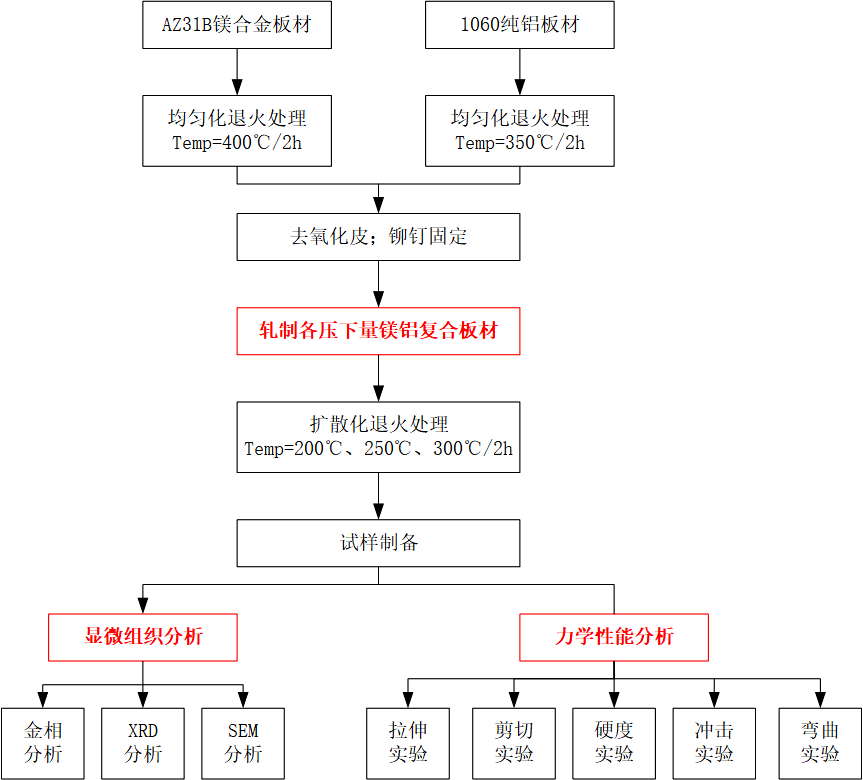
\includegraphics[width=0.5\textwidth]{images/liuchengtu.png}
	\caption{实验流程图}
	\label{fig:liuchengtu}
\end{figure}
\subsection{实验材料}
实验所采用的原始材料为商用AZ31B镁合金铸轧板材和1060铝板材。合金原材料采用连续铸轧工艺生产,生产工序经过配料/熔炼/静置/放料/连续铸轧等流程,由于原材料板材较大,采用剪板机进行切割取样。\par
公式格式:
\begin{equation}
\label{equ:maxwell}
    \begin{cases}
    \nabla\times\vec{E}=-\frac{\partial\vec{B}}{\partial t}\\
    \nabla\times\vec{H}=\vec{J_v}+\frac{\partial\vec{D}}{\partial t}\\
    \nabla\cdot\vec{D}=\rho_v\\
    \nabla\cdot\vec{B}=0
    \end{cases}\quad
    \begin{cases}
    \vec{D}=\epsilon\vec{E}\\
    \vec{B}=\mu\vec{H}\\
    \vec{J_v}=\sigma\vec{E}
    \end{cases}  
\end{equation}

表格格式:
\begin{table}[H]
    \centering
    \caption{一个表格}
    \zihao{5}
    \label{tab:all_parameters}
    \begin{tabular}{c c c l}
    \toprule[1.5pt]
    参数          & 数值         & 单位   & 备注     \\ 
    \midrule[0.5pt]
    $A$         & 2132   & 1      & A参数 \\
    $B$         & 3423   & 1      & B参数 \\ 
    $C$         & 1232   & 1      & C参数 \\ 
    $D$         & 1234   & μm     & D参数 \\
    $\alpha$    & 11.1   & cm     & α参数 \\
    $\beta$     & 123.3  & km     & β参数 \\       
    \bottomrule[1.5pt]
    \end{tabular}
\end{table}

\clearpage
\section{系统总体设计}

	系统总体结构组成如\Cref{overall_structure}所示,省略一段文字省略一段文字省略一段文字省略一段文字省略一段文字省略一段文字省略一段文字省略一段文字省略一段文字省略一段文字省略一段文字省略一段文字省略一段文字省
		
	\begin{figure}[H]
		\centering
		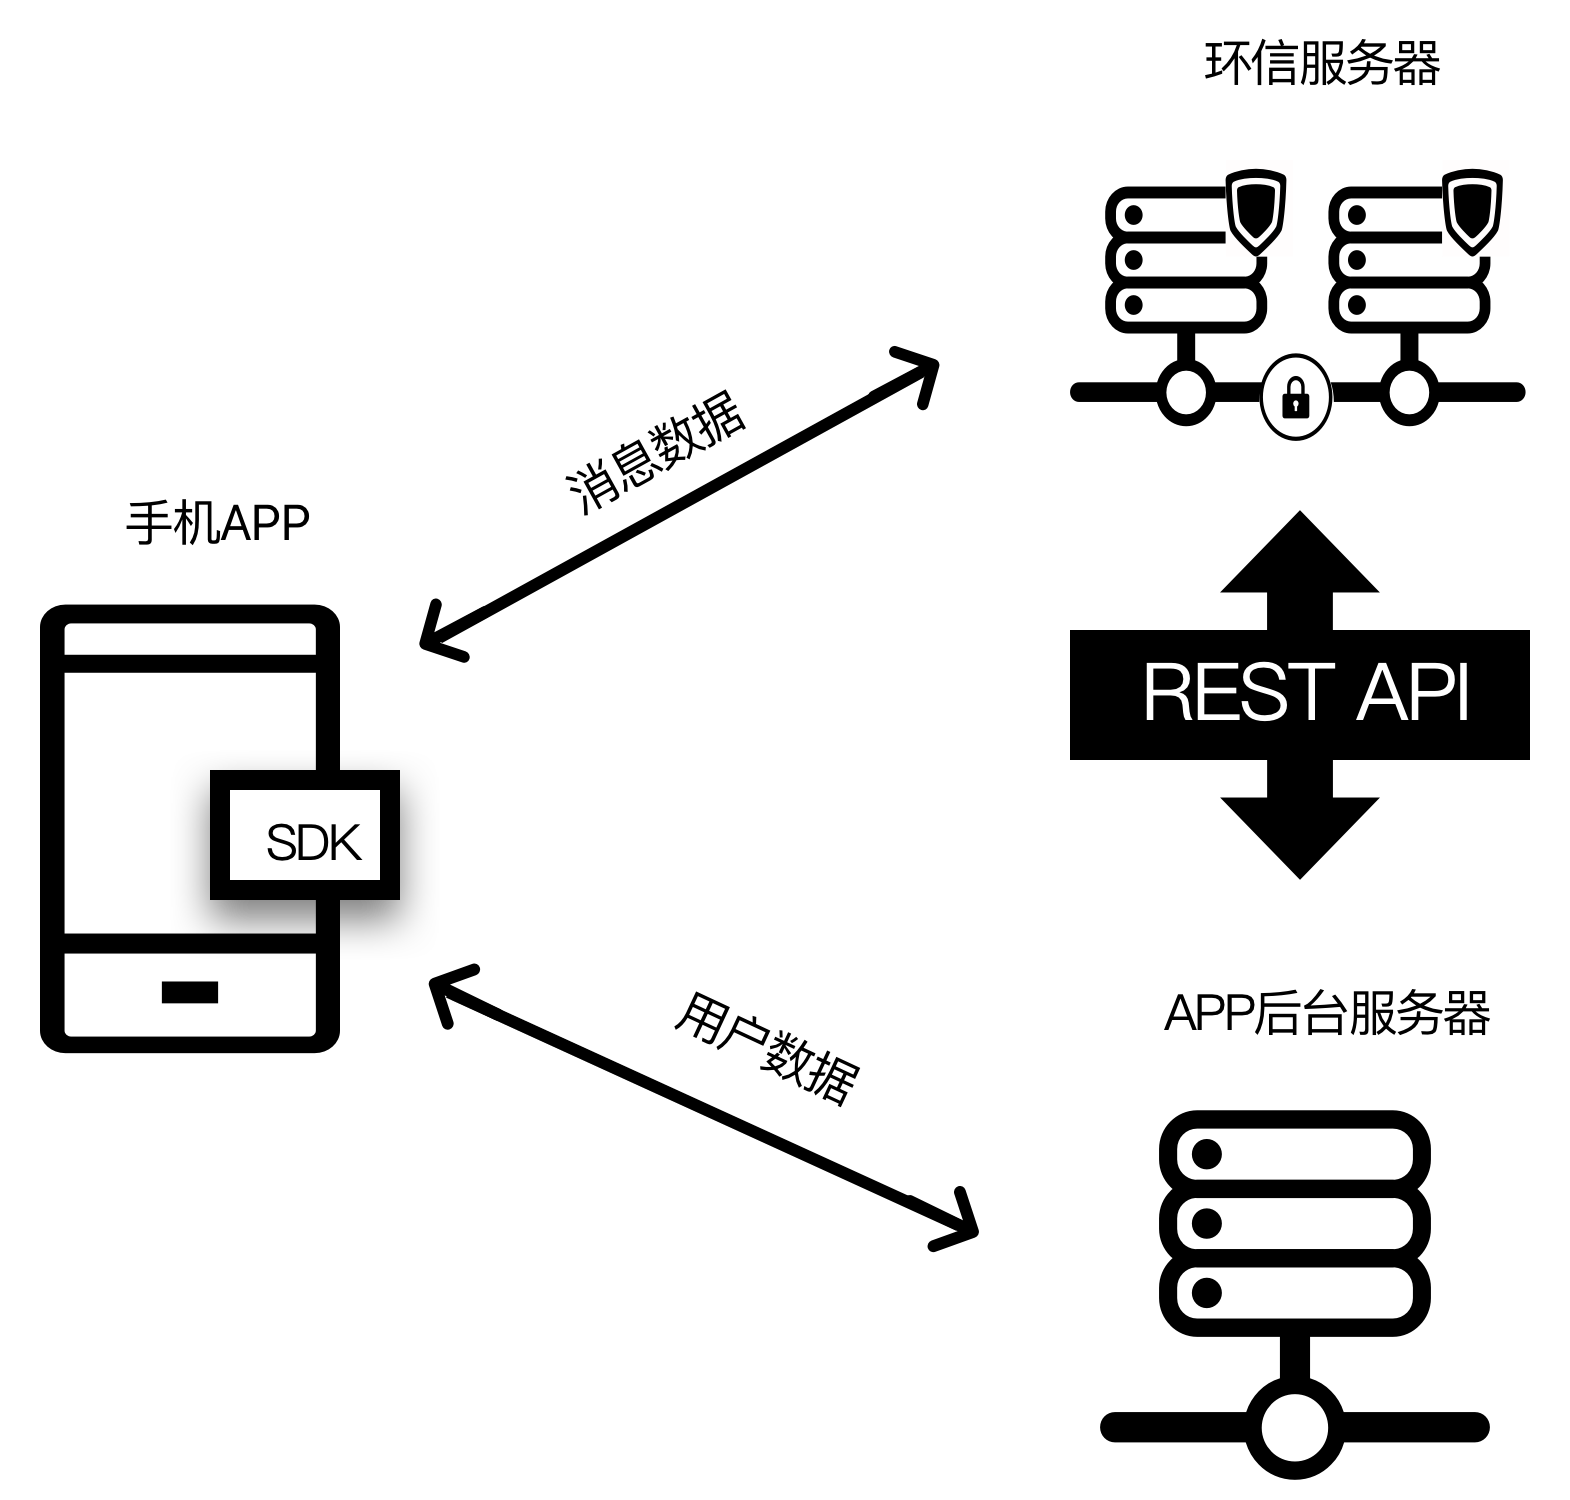
\includegraphics[width=0.80\textwidth]{images/all_design}
		\caption{系统总体结构组成}
		\label{overall_structure}
	\end{figure}
	
	\subsection{服务端总体设计}
	
		服务端的实现省略一段文字省略一段文字省略一段文字省略一段文字省略一段文字省略一段文字省略一段文字省略一段文字省略一段文字省略一段文字省略一段文字省略一段文字省略一段文字省		  
		  
		 省略一段文字省略一段文字省略一段文字省略一段文字省略一段文字省略一段文字省略一段文字省略一段文字省略一段文字省略一段文字省略一段文字省略一段文字省略一段文字省
		 
		  		  
		  
	\subsection{客户端总体设计}
		
		客户端采用分层的架构进行设计,上层实现依赖于下层设计\scite{cite_分层设计},自下而上分为基础层、数据层、组件层、表现层、应用层,整体设计结构如\Cref{mobile_overall_design}所示。
	
	\begin{figure}[H]
		\centering
		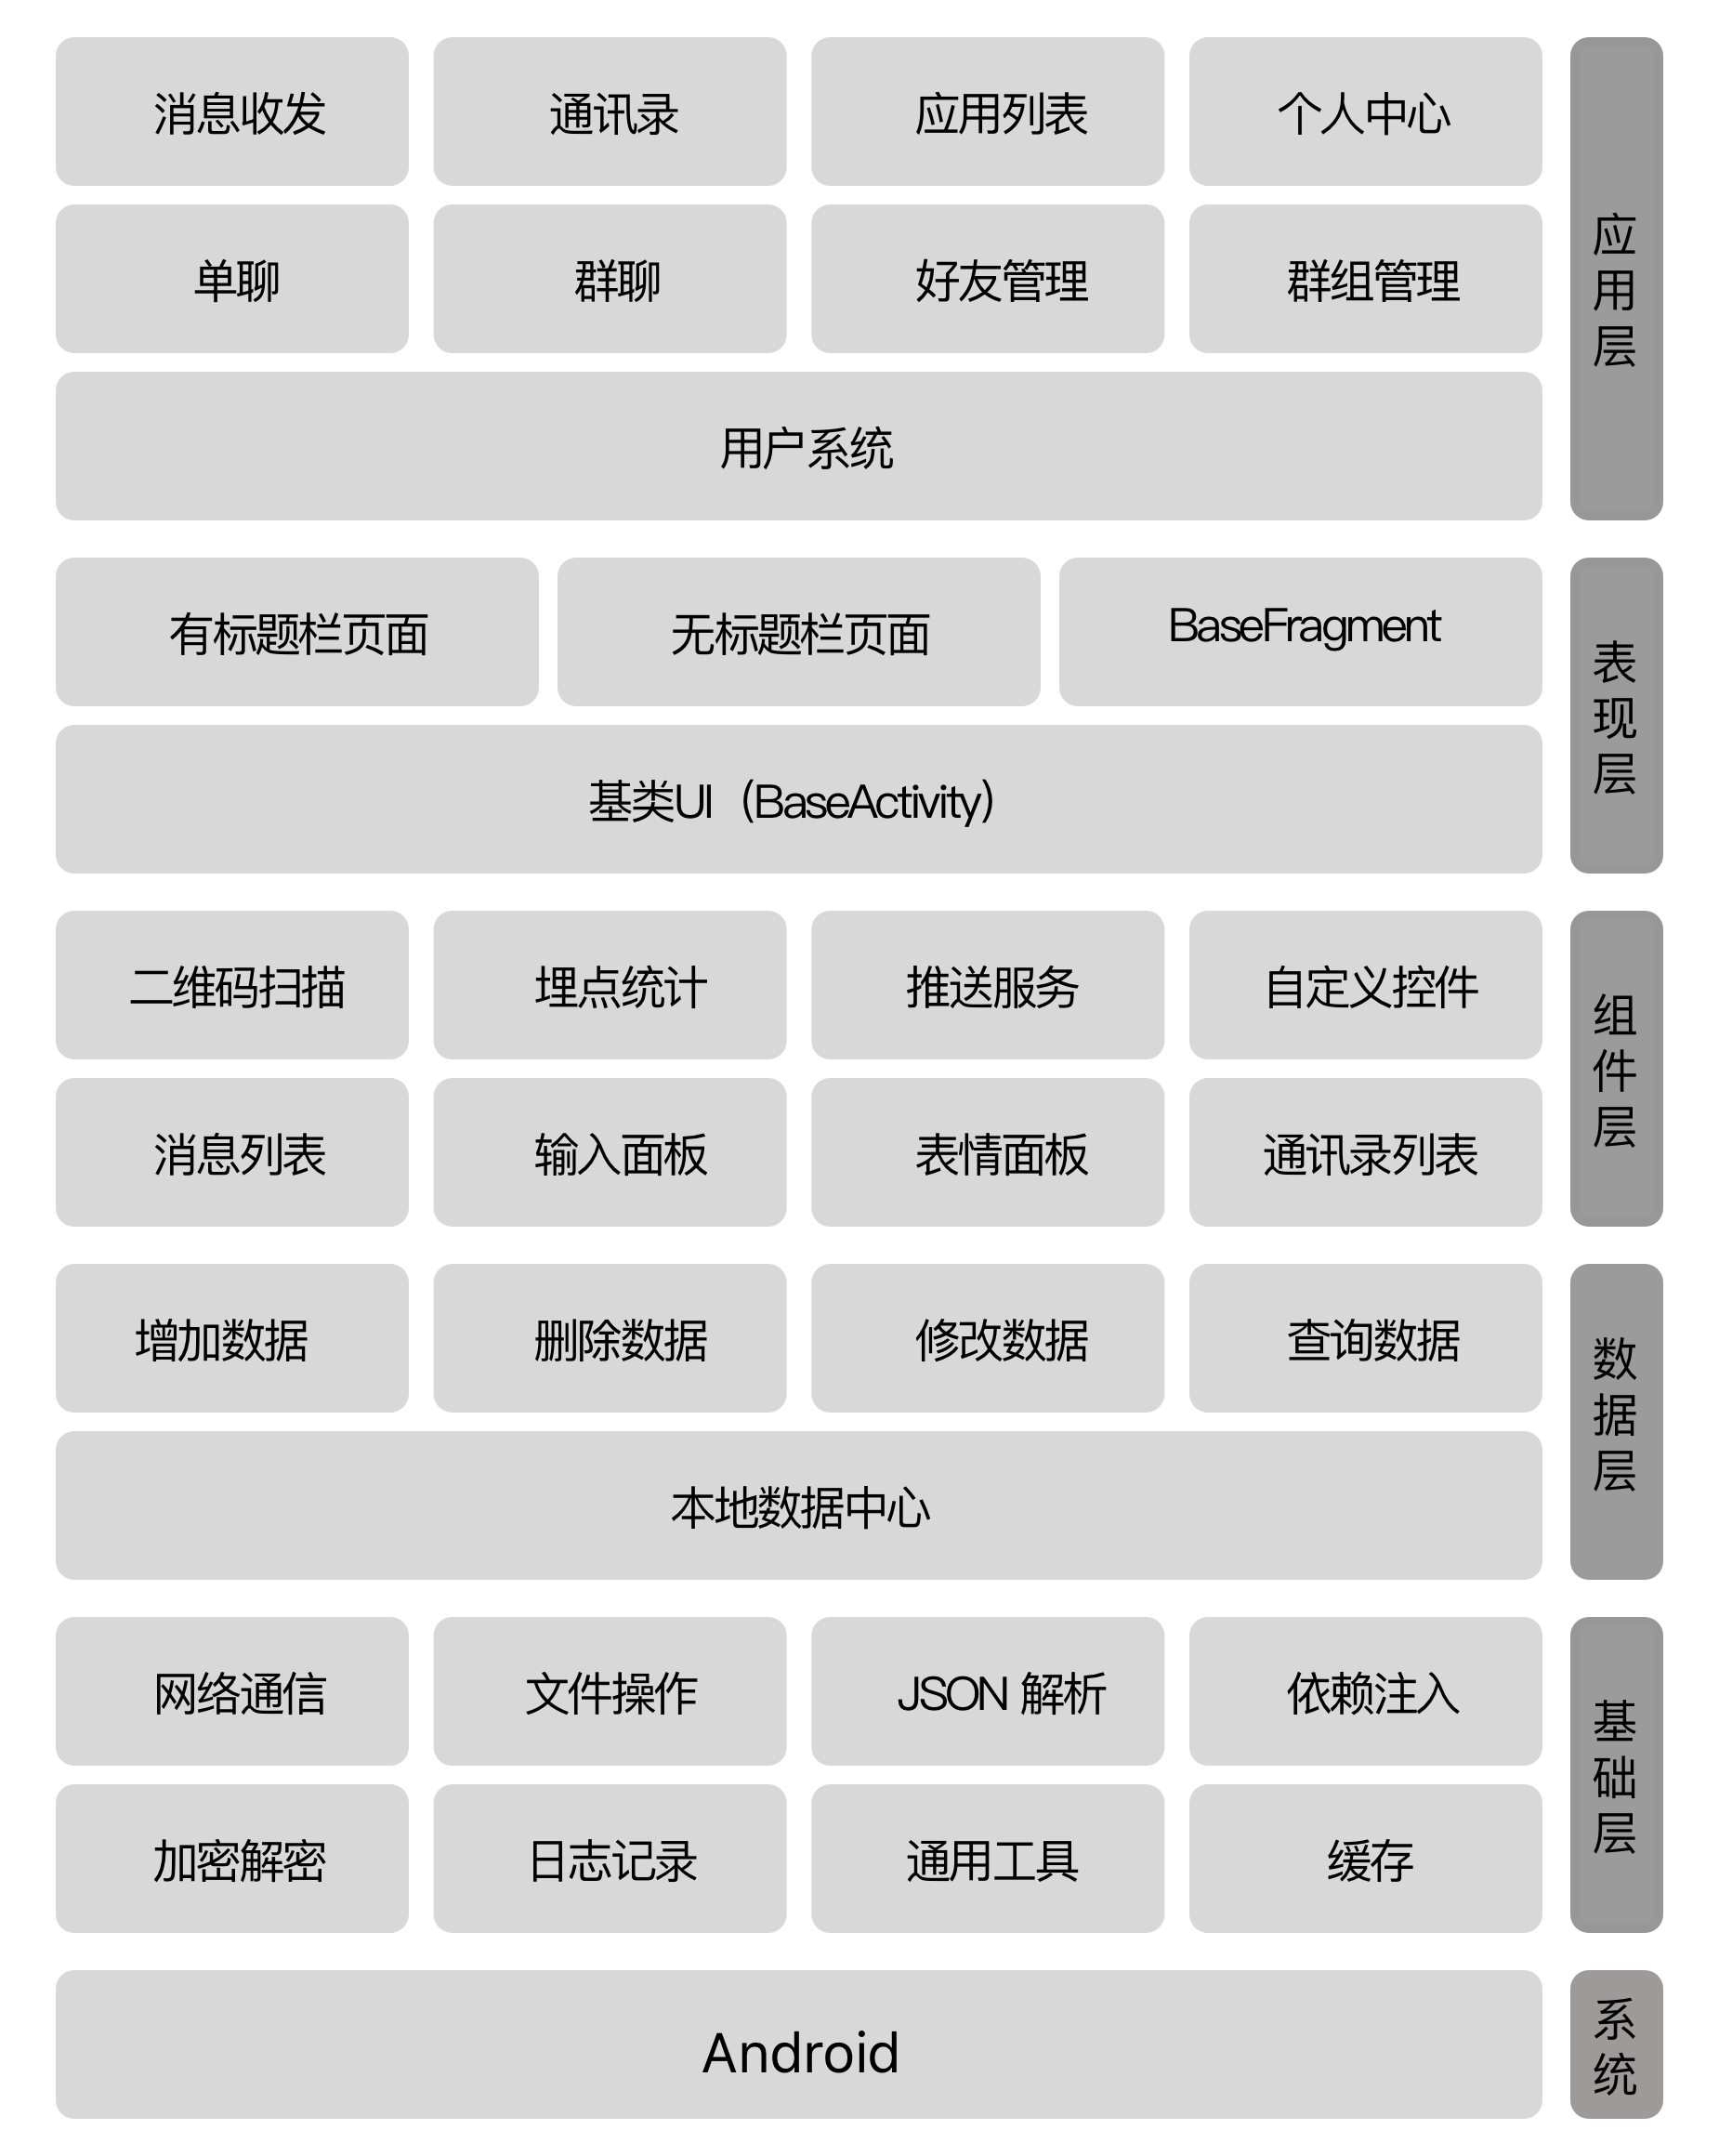
\includegraphics[width=0.95\textwidth]{images/mobile_design}
		\caption{移动端总体设计结构}
		\label{mobile_overall_design}
	\end{figure}


	\begin{enumerate}[fullwidth,itemindent=2em,listparindent=2em]
	
		\item 设计概述
		
		省略一段文字省略一段文字省略一段文字省略一段文字省略一段文字省略一段文字省略一段文字省略一段文字省略一段文字省略一段文字省略一段文字省略一段文字省略一段文字省
		
		省略一段文字省略一段文字省略一段文字省略一段文字省略一段文字省略一段文字省略一段文字省略一段文字省略一段文字省略一段文字省略一段文字省略一段文字省略一段文字省
		
		\item 设计概述
		
		省略一段文字省略一段文字省略一段文字省略一段文字省略一段文字省略一段文字省略一段文字省略一段文字省略一段文字省略一段文字省略一段文字省略一段文字省略一段文字省
		
		省略一段文字省略一段文字省略一段文字省略一段文字省略一段文字省略一段文字省略一段文字省略一段文字省略一段文字省略一段文字省略一段文字省略一段文字省略一段文字省

		\item 设计概述
		
		省略一段文字省略一段文字省略一段文字省略一段文字省略一段文字省略一段文字省略一段文字省略一段文字省略一段文字省略一段文字省略一段文字省略一段文字省略一段文字省
		
		省略一段文字省略一段文字省略一段文字省略一段文字省略一段文字省略一段文字省略一段文字省略一段文字省略一段文字省略一段文字省略一段文字省略一段文字省略一段文字省

			
		

	\end{enumerate}

	\subsection{数据库总体设计}

		
		省略一段文字省略一段文字省略一段文字省略一段文字省略一段文字省略一段文字省略一段文字省略一段文字省略一段文字省略一段文字省略一段文字省,表格使用,表格使用,表格使用,表格使用,表格使用,表格使用,如\Cref{tab:db_table_user}所示。
	
		\begin{table}[H]
		\centering
		\caption{\ \ User 用户表}
		\zihao{5}
		\label{tab:db_table_user}
		\begin{tabular}{p{0.21\textwidth}p{0.21\textwidth}p{0.21\textwidth}p{0.21\textwidth}}
		\toprule[1.5pt]
		字段          & 数据类型         & 字段含义   & 约束条件     \\ 
		\midrule[0.75pt]
		id          & INT(11)      & 用户ID & 主键、非空、自增 \\
		im\_id      & VARCHAR(256) & 环信ID & 唯一       \\ 
		account     & VARCHAR(45)  & 用户名  & 唯一       \\ 
		nick\_name  & VARCHAR(100) & 昵称   & 无        \\
		password    & VARCHAR(256) & 密码   & 非空       \\ 
		email       & VARCHAR(45)  & 邮箱   & 无        \\
		mobile      & VARCHAR(45)  & 手机号  & 唯一        \\ 
		sex         & INT(11)      & 性别   & 无        \\ 
		signature   & VARCHAR(512) & 签名   & 无        \\
		avatar      & VARCHAR(256) & 头像   & 无        \\
		is\_deleted & TINYINT(4)   & 删除标志 & 无        \\ 
		\bottomrule[1.5pt]
		\end{tabular}
		\end{table}
		
 \clearpage
\section{系统详细设计}

	系统详细设计实现省略一段文字省略一段文字省略一段文字省略一段文字省略一段文字省略一段文字省略一段文字省略一段文字省略一段文字省略一段文字省略一段文字省略一段文字省略一段文字省省略一段文字省略一段文字省略一段文字省略一段文字省略一段文字省略一段文字省略一段文字省略一段文字省略一段文字省略一段文字省略一段文字省略一段文字省略一段文字省

  \subsection{基础层详细设计}
	
   	\subsubsection{网络通信的实现}

		实现省略一段文字省略一段文字省略一段文字省略一段文字省略一段文字省略一段文字省略一段文字省略一段文字省略一段文字省略一段文字省略一段文字省略一段文字省略一段文字省省略一段文字省略一段文字省略一段文字省略一段文字省略一段文字省略一段文字省略一段文字省略一段文字省略一段文字省略一段文字省略一段文字省略一段文字省略一段文字省

		
		这里以\Cref{code_api_service} 为例,代码块使用示例
		
		
		\begin{lstlisting}[caption=APIService , label=code_api_service]
 /** 
  * 登录 
  */
 @POST("user/login")
 Call<APIResponse<LoginResponse>> login(@Body LoginRequest request);

 /** 
  * 获取单个用户详细信息
  */
 @GET("user/{imid}/info")
 Call<APIResponse<UserInfo>> getUserInfo(@Path("imid") String imId);
 
		\end{lstlisting}                 

	
			
   	\subsubsection{日志记录的实现}
    
    实现省略一段文字省略一段文字省略一段文字省略一段文字省略一段文字省略一段文字省略一段文字省略一段文字省略一段文字省略一段文字省略一段文字省略一段文字省略一段文字省省略一段文字省略一段文字省略一段文字省略一段文字省略一段文字省略一段文字省略一段文字省略一段文字省略一段文字省略一段文字省略一段文字省略一段文字省略一段文字省日志记录输出样式如\Cref{img_log_sample}所示。
    
    \begin{figure}[H]
    	\centering
    	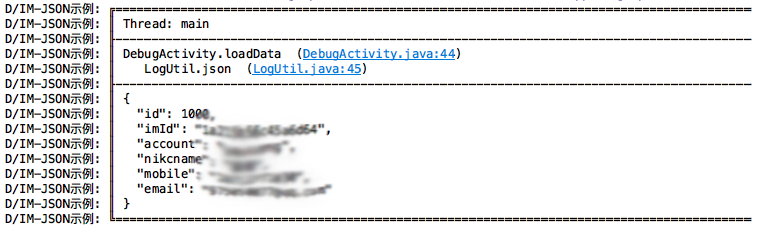
\includegraphics[width=0.95\textwidth]{images/log_sample}
    	\caption{日志信息示例}
    	\label{img_log_sample}
    \end{figure}
    
    
   	\subsubsection{加密解密的实现}
    
    实现省略一段文字省略一段文字省略一段文字省略一段文字省略一段文字省略一段文字省略一段文字省略一段文字省略一段文字省略一段文字省略一段文字省略一段文字省略一段文字省省略一段文字省略一段文字省略一段文字省略一段文字省略一段文字省略一段文字省略一段文字省略一段文字省略一段文字省略一段文字省略一段文字省略一段文字省略一段文字省
        
   	\subsubsection{缓存的实现}
   	
   	实现省略一段文字省略一段文字省略一段文字省略一段文字省略一段文字省略一段文字省略一段文字省略一段文字省略一段文字省略一段文字省略一段文字省略一段文字省略一段文字省省略一段文字省略一段文字省略一段文字省略一段文字省略一段文字省略一段文字省略一段文字省略一段文字省略一段文字省略一段文字省略一段文字省略一段文字省略一段文字省
   	   	
   	\subsubsection{文件操作工具的实现}
   	
   	文件操作模块定义了全局工具类 FileUtil,内部实现了常用的文件操作方法以及格式化输出文件大小的方法。常用文件操作方法包含判断文件是否存在、读文件、写文件、移动文件、复制文件、删除文件、创建文件、文件重命名、获取文件名称、判断是否有文件夹、调用系统方式打开文件、将字符串以不同形式的编码写入文件中。格式化文件大小主要是将文件的大小转换为更直观的形式,如:15KB、0.38M、1.52G。
   	
   	\subsubsection{JSON解析的实现}

	实现省略一段文字省略一段文字省略一段文字省略一段文字省略一段文字省略一段文字省略一段文字省略一段文字省略一段文字省略一段文字省略一段文字省略一段文字省略一段文字省省略一段文字省略一段文字省略一段文字省略一段文字省略一段文字省略一段文字省略一段文字省略一段文字省略一段文字省略一段文字省略一段文字省略一段文字省略一段文字省
	
  \subsection{数据层详细设计}

	实现省略一段文字省略一段文字省略一段文字省略一段文字省略一段文字省略一段文字省略一段文字省略一段文字省略一段文字省略一段文字省略一段文字省略一段文字省略一段文字省省略一段文字省略一段文字省略一段文字省略一段文字省略一段文字省略一段文字省略一段文字省略一段文字省略一段文字省略一段文字省略一段文字省略一段文字省略一段文字省
		 
	
	实现省略一段文字省略一段文字省略一段文字省略一段文字省略一段文字省略一段文字省略一段文字省略一段文字省略一段文字省略一段文字省略一段文字省略一段文字省略一段文字省省略一段文字省略一段文字省略一段文字省略一段文字省略一段文字省略一段文字省略一段文字省略一段文字省略一段文字省略一段文字省略一段文字省略一段文字省略一段文字省
	
	
  \subsection{组件层详细设计}

   	\subsubsection{二维码扫描的实现}
   	
	实现省略一段文字省略一段文字省略一段文字省略一段文字省略一段文字省略一段文字省略一段文字省略一段文字省略一段文字省略一段文字省略一段文字省略一段文字省略一段文字省省略一段文字省略一段文字省略一段文字省略一段文字省略一段文字省略一段文字省略一段文字省略一段文字省略一段文字省略一段文字省略一段文字省略一段文字省略一段文字省

   	\subsubsection{消息列表的实现}
	
	实现省略一段文字省略一段文字省略一段文字省略一段文字省略一段文字省略一段文字省略一段文字省略一段文字省略一段文字省略一段文字省略一段文字省略一段文字省略一段文字省省略一段文字省略一段文字省略一段文字省略一段文字省略一段文字省略一段文字省略一段文字省略一段文字省略一段文字省略一段文字省略一段文字省略一段文字省略一段文字省
	
   	\subsubsection{输入面板的实现}
   	
   	实现省略一段文字省略一段文字省略一段文字省略一段文字省略一段文字省略一段文字省略一段文字省略一段文字省略一段文字省略一段文字省略一段文字省略一段文字省略一段文字省省略一段文字省略一段文字省略一段文字省略一段文字省略一段文字省略一段文字省略一段文字省略一段文字省略一段文字省略一段文字省略一段文字省略一段文字省略一段文字省,输入面板具体样式如\Cref{input_panel}所示。
   	
   	\begin{figure}[H]
		\centering
		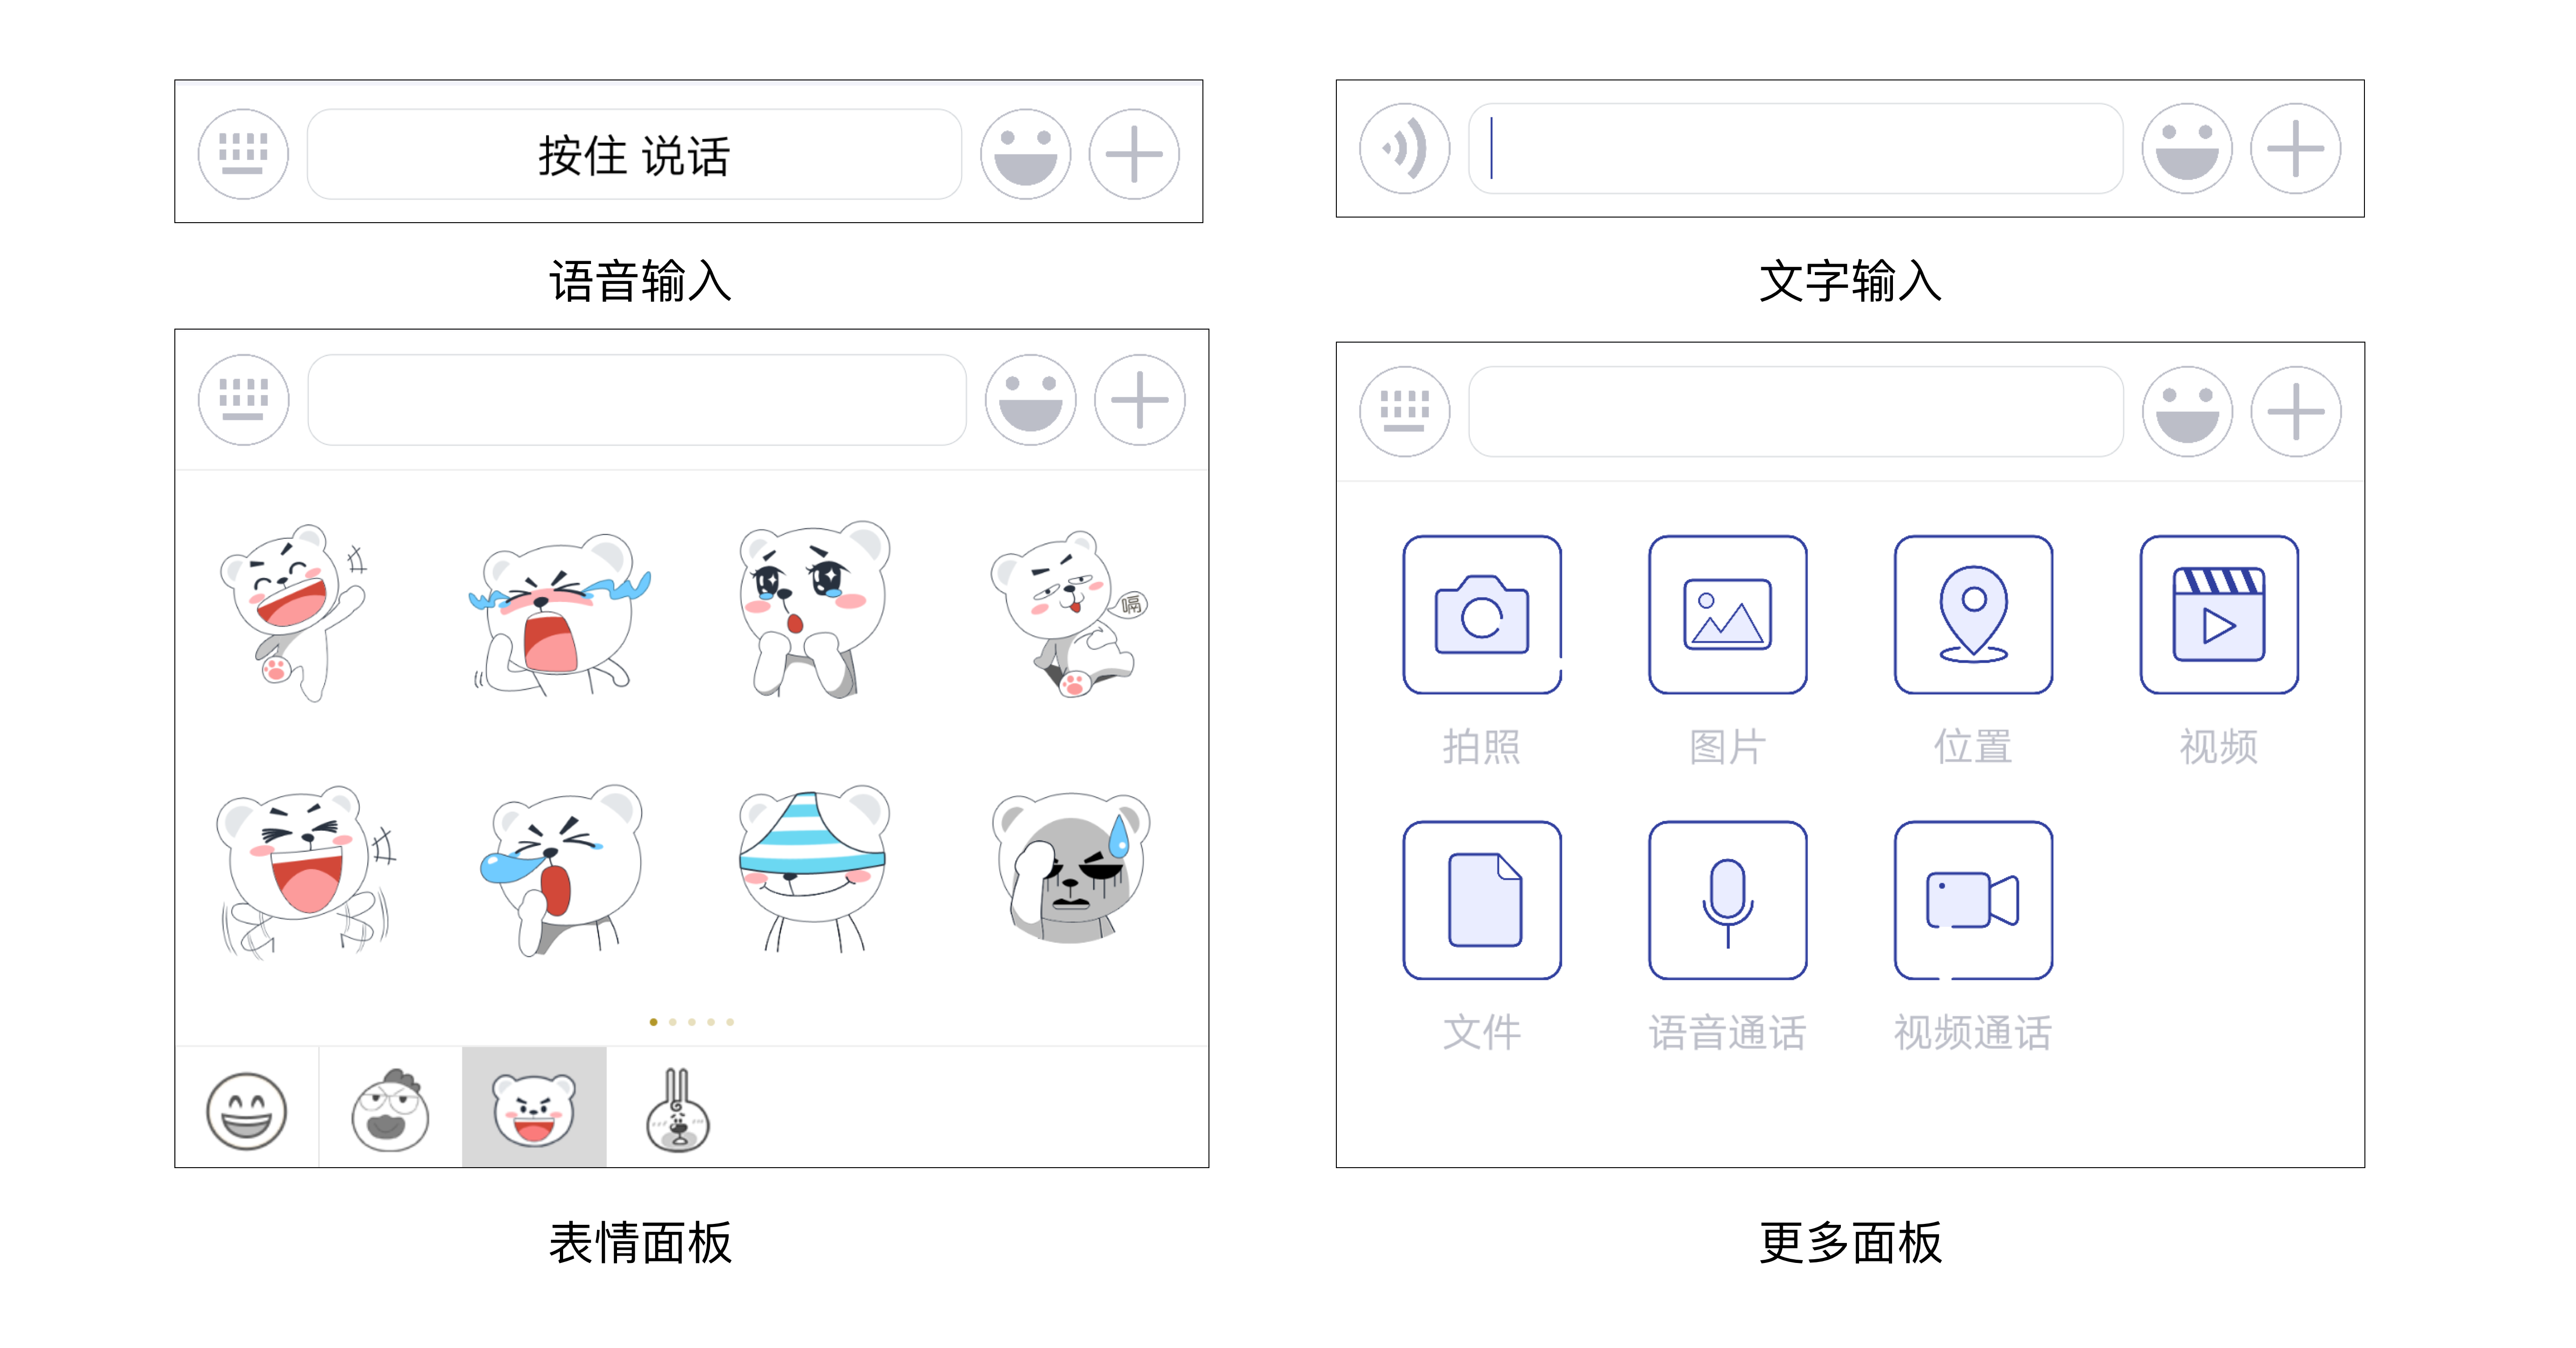
\includegraphics[width=0.95\textwidth]{images/input_panel}
		\caption{输入面板样式}
		\label{input_panel}
	\end{figure}
	
	
   	\subsubsection{表情面板的实现}
   	
   	实现省略一段文字省略一段文字省略一段文字省略一段文字省略一段文字省略一段文字省略一段文字省略一段文字省略一段文字省略一段文字省略一段文字省略一段文字省略一段文字省省略一段文字省略一段文字省略一段文字省略一段文字省略一段文字省略一段文字省略一段文字省略一段文字省略一段文字省略一段文字省略一段文字省略一段文字省略一段文字省   	
   	   	   	
   	\subsubsection{更多面板的实现}
   	
   	实现省略一段文字省略一段文字省略一段文字省略一段文字省略一段文字省略一段文字省略一段文字省略一段文字省略一段文字省略一段文字省略一段文字省略一段文字省略一段文字省省略一段文字省略一段文字省略一段文字省略一段文字省略一段文字省略一段文字省略一段文字省略一段文字省略一段文字省略一段文字省略一段文字省略一段文字省略一段文字省
   	    
   	\subsubsection{通讯录列表的实现}
   	
   	实现省略一段文字省略一段文字省略一段文字省略一段文字省略一段文字省略一段文字省略一段文字省略一段文字省略一段文字省略一段文字省略一段文字省略一段文字省略一段文字省省略一段文字省略一段文字省略一段文字省略一段文字省略一段文字省略一段文字省略一段文字省略一段文字省略一段文字省略一段文字省略一段文字省略一段文字省略一段文字省
    
	\subsubsection{埋点统计的实现}
	
	实现省略一段文字省略一段文字省略一段文字省略一段文字省略一段文字省略一段文字省略一段文字省略一段文字省略一段文字省略一段文字省略一段文字省略一段文字省略一段文字省省略一段文字省略一段文字省略一段文字省略一段文字省略一段文字省略一段文字省略一段文字省略一段文字省略一段文字省略一段文字省略一段文字省略一段文字省略一段文字省
		
          

  \subsection{表现层详细设计}
	
	  \subsubsection{Activity 基类的实现}
	  
		实现省略一段文字省略一段文字省略一段文字省略一段文字省略一段文字省略一段文字省略一段文字省略一段文字省略一段文字省略一段文字省略一段文字省略一段文字省略一段文字省省略一段文字省略一段文字省略一段文字省略一段文字省略一段文字省略一段文字省略一段文字省略一段文字省略一段文字省略一段文字省略一段文字省略一段文字省略一段文字省
	  		

	  
	  	  
	  \subsubsection{Fragment 基类的实现}
	  
		实现省略一段文字省略一段文字省略一段文字省略一段文字省略一段文字省略一段文字省略一段文字省略一段文字省略一段文字省略一段文字省略一段文字省略一段文字省略一段文字省省略一段文字省略一段文字省略一段文字省略一段文字省略一段文字省略一段文字省略一段文字省略一段文字省略一段文字省略一段文字省略一段文字省略一段文字省略一段文字省
		

  \subsection{应用层详细设计}
  	
		\subsubsection{用户系统的实现}
		
		实现省略一段文字省略一段文字省略一段文字省略一段文字省略一段文字省略一段文字省略一段文字省略一段文字省略一段文字省略一段文字省略一段文字省略一段文字省略一段文字省省略一段文字省略一段文字省略一段文字省略一段文字省略一段文字省略一段文字省略一段文字省略一段文字省略一段文字省略一段文字省略一段文字省略一段文字省略一段文字省
		
		\subsubsection{聊天功能的实现}
		
		实现省略一段文字省略一段文字省略一段文字省略一段文字省略一段文字省略一段文字省略一段文字省略一段文字省略一段文字省略一段文字省略一段文字省略一段文字省略一段文字省省略一段文字省略一段文字省略一段文字省略一段文字省略一段文字省略一段文字省略一段文字省略一段文字省略一段文字省略一段文字省略一段文字省略一段文字省略一段文字省
				
	 	\subsubsection{好友管理的实现}
	 	
	 	实现省略一段文字省略一段文字省略一段文字省略一段文字省略一段文字省略一段文字省略一段文字省略一段文字省略一段文字省略一段文字省略一段文字省略一段文字省略一段文字省省略一段文字省略一段文字省略一段文字省略一段文字省略一段文字省略一段文字省略一段文字省略一段文字省略一段文字省略一段文字省略一段文字省略一段文字省略一段文字省
	 	
		\subsubsection{群组管理的实现}
		
		实现省略一段文字省略一段文字省略一段文字省略一段文字省略一段文字省略一段文字省略一段文字省略一段文字省略一段文字省略一段文字省略一段文字省略一段文字省略一段文字省省略一段文字省略一段文字省略一段文字省略一段文字省略一段文字省略一段文字省略一段文字省略一段文字省略一段文字省略一段文字省略一段文字省略一段文字省略一段文字省
		
		\subsubsection{通讯录的实现}
		
		实现省略一段文字省略一段文字省略一段文字省略一段文字省略一段文字省略一段文字省略一段文字省略一段文字省略一段文字省略一段文字省略一段文字省略一段文字省略一段文字省省略一段文字省略一段文字省略一段文字省略一段文字省略一段文字省略一段文字省略一段文字省略一段文字省略一段文字省略一段文字省略一段文字省略一段文字省略一段文字省
		
		\subsubsection{应用列表的实现}
		
		实现省略一段文字省略一段文字省略一段文字省略一段文字省略一段文字省略一段文字省略一段文字省略一段文字省略一段文字省略一段文字省略一段文字省略一段文字省略一段文字省省略一段文字省略一段文字省略一段文字省略一段文字省略一段文字省略一段文字省略一段文字省略一段文字省略一段文字省略一段文字省略一段文字省略一段文字省略一段文字省GridView更新。
		
		\subsubsection{个人中心的实现}
		
		实现省略一段文字省略一段文字省略一段文字省略一段文字省略一段文字省略一段文字省略一段文字省略一段文字省略一段文字省略一段文字省略一段文字省略一段文字省略一段文字省省略一段文字省略一段文字省略一段文字省略一段文字省略一段文字省略一段文字省略一段文字省略一段文字省略一段文字省略一段文字省略一段文字省略一段文字省略一段文字省

 \clearpage
\section{系统部署与测试}
	\subsection{服务端部署}
 
	实现省略一段文字省略一段文字省略一段文字省略一段文字省略一段文字省略一段文字省略一段文字省略一段文字省略一段文字省略一段文字省略一段文字省略一段文字省略一段文字省省略一段文字省略一段文字省略一段文字省略一段文字省略一段文字省略一段文字省略一段文字省略一段文字省略一段文字省略一段文字省略一段文字省略一段文字省略一段文字省
	
	 
	\subsection{客户端测试}
	
	\subsubsection{单元测试}
	
	实现省略一段文字省略一段文字省略一段文字省略一段文字省略一段文字省略一段文字省略一段文字省略一段文字省略一段文字省略一段文字省略一段文字省略一段文字省略一段文字省省略一段文字省略一段文字省略一段文字省略一段文字省略一段文字省略一段文字省略一段文字省略一段文字省略一段文字省略一段文字省略一段文字省略一段文字省略一段文字省

 	\subsubsection{功能测试}
 	
 	实现省略一段文字省略一段文字省略一段文字省略一段文字省略一段文字省略一段文字省略一段文字省略一段文字省略一段文字省略一段文字省略一段文字省略一段文字省略一段文字省省略一段文字省略一段文字省略一段文字省略一段文字省略一段文字省略一段文字省略一段文字省略一段文字省略一段文字省略一段文字省略一段文字省略一段文字省略一段文字省 	
 	
 	\subsubsection{深度兼容测试}
	
	实现省略一段文字省略一段文字省略一段文字省略一段文字省略一段文字省略一段文字省略一段文字省略一段文字省略一段文字省略一段文字省略一段文字省略一段文字省略一段文字省省略一段文字省略一段文字省略一段文字省略一段文字省略一段文字省略一段文字省略一段文字省略一段文字省略一段文字省略一段文字省略一段文字省略一段文字省略一段文字省


\clearpage
\section*{结\ \ \ \ \ \ \ \ 论}
\addcontentsline{toc}{section}{结\ \ \ \ \ \ \ \ 论}


	实现省略一段文字省略一段文字省略一段文字省略一段文字省略一段文字省略一段文字省略一段文字省略一段文字省略一段文字省略一段文字省略一段文字省略一段文字省略一段文字省省略一段文字省略一段文字省略一段文字省略一段文字省略一段文字省略一段文字省略一段文字省略一段文字省略一段文字省略一段文字省略一段文字省略一段文字省略一段文字省。总体上,完成了以下工作:
	
	\begin{enumerate}
	
		\item 调研了...
		
		\item 调研...
		
		\item 设计...
				
		\item 依据...	
		
		\item 对整个系统...

		 
	\end{enumerate}
	
	
	实现省略一段文字省略一段文字省略一段文字省略一段文字省略一段文字省略一段文字省略一段文字省略一段文字省略一段文字省略一段文字省略一段文字省略一段文字省略一段文字省省略一段文字省略一段文字省略一段文字省略一段文字省略一段文字省略一段文字省略一段文字省略一段文字省略一段文字省略一段文字省略一段文字省略一段文字省略一段文字省
\section*{致\ \ \ \ \ \ \ \ 谢}
\addcontentsline{toc}{section}{致\ \ \ \ \ \ \ \ 谢}

	实现省略一段文字省略一段文字省略一段文字省略一段文字省略一段文字省略一段文字省略一段文字省略一段文字省略一段文字省略一段文字省略一段文字省略一段文字省略一段文字省省略一段文字省略一段文字省略一段文字省略一段文字省略一段文字省略一段文字省略一段文字省略一段文字省略一段文字省略一段文字省略一段文字省略一段文字省略一段文字省

% \bibliographystyle{IEEEtran}
\bibliographystyle{gbt7714-2005}
% \bibliographystyle{thu}
% \bibliographystyle{cqu}
\nocite{*}
\addcontentsline{toc}{section}{参考文献}
\renewcommand\bibnumfmt[1]{\makebox[0.9cm][l]{[#1]}}
\setlength{\bibhang}{0em}

\bibliography{citation}
%\setlength{\bibindent}{5cm}

\appendix
% \renewcommand{\appendixname}{附录~\Alph{section}}
% \renewcommand{\appendixtocname}{附录}
% \addappheadtotoc
% \renewcommand{\appendixpagename}{\centering 附录}
% \appendixpage

% \begin{appendices}

% \heiti
% \zihao{3}

\section*{附\ \ \ \ \ \ \ \ 录}

\addcontentsline{toc}{section}{附\ \ \ \ \ \ \ \ 录}

\renewcommand{\thesubsection}{附录\Alph{subsection}}
% \renewcommand\thetable{\thesection.\arabic{table}}
% \renewcommand\thefigure{\arabic{figure}}

\newcommand{\appendsection}[1]{\titleformat*{\subsection}{}\zihao{-4}\heiti\subsection{} {\centering\paragraph{#1}\mbox{}\\}\songti}
\newcommand{\appendchn}[1]{\titleformat*{\subsection}{}\zihao{-4}\heiti\subsection*{中文译文\Alph{subsection}} {\centering\paragraph{#1}\mbox{}\\}\songti}

% \renewcommand{\figurename}{图 A.}
% \setcounter{figure}{0}

% \titlespacing*{\subsection}{-20pt}{*1.5}{*1.1}


\appendsection{Android, the world's most popular mobile platform}

	实现省略一段文字省略一段文字省略一段文字省略一段文字省略一段文字省略一段文字省略一段文字省略一段文字省略一段文字省略一段文字省略一段文字省略一段文字省略一段文字省省略一段文字省略一段文字省略一段文字省略一段文字省略一段文字省略一段文字省略一段文字省略一段文字省略一段文字省略一段文字省略一段文字省略一段文字省略一段文字省



\appendchn{Android,世界上最受欢迎的移动平台}

	实现省略一段文字省略一段文字省略一段文字省略一段文字省略一段文字省略一段文字省略一段文字省略一段文字省略一段文字省略一段文字省略一段文字省略一段文字省略一段文字省省略一段文字省略一段文字省略一段文字省略一段文字省略一段文字省略一段文字省略一段文字省略一段文字省略一段文字省略一段文字省略一段文字省略一段文字省略一段文字省


\appendsection{Android Application Fundamentals}

	实现省略一段文字省略一段文字省略一段文字省略一段文字省略一段文字省略一段文字省略一段文字省略一段文字省略一段文字省略一段文字省略一段文字省略一段文字省略一段文字省省略一段文字省略一段文字省略一段文字省略一段文字省略一段文字省略一段文字省略一段文字省略一段文字省略一段文字省略一段文字省略一段文字省略一段文字省略一段文字省

\subsubsection*{Application Components}

	实现省略一段文字省略一段文字省略一段文字省略一段文字省略一段文字省略一段文字省略一段文字省略一段文字省略一段文字省略一段文字省略一段文字省略一段文字省略一段文字省省略一段文字省略一段文字省略一段文字省略一段文字省略一段文字省略一段文字省略一段文字省略一段文字省略一段文字省略一段文字省略一段文字省略一段文字省略一段文字省components:

\subsubsection*{Activities}

	实现省略一段文字省略一段文字省略一段文字省略一段文字省略一段文字省略一段文字省略一段文字省略一段文字省略一段文字省略一段文字省略一段文字省略一段文字省略一段文字省省略一段文字省略一段文字省略一段文字省略一段文字省略一段文字省略一段文字省略一段文字省略一段文字省略一段文字省略一段文字省略一段文字省略一段文字省略一段文字省	
		
\subsubsection*{Services}

	实现省略一段文字省略一段文字省略一段文字省略一段文字省略一段文字省略一段文字省略一段文字省略一段文字省略一段文字省略一段文字省略一段文字省略一段文字省略一段文字省省略一段文字省略一段文字省略一段文字省略一段文字省略一段文字省略一段文字省略一段文字省略一段文字省略一段文字省略一段文字省略一段文字省略一段文字省略一段文字省

\subsubsection*{Broadcast receivers}

	实现省略一段文字省略一段文字省略一段文字省略一段文字省略一段文字省略一段文字省略一段文字省略一段文字省略一段文字省略一段文字省略一段文字省略一段文字省略一段文字省省略一段文字省略一段文字省略一段文字省略一段文字省略一段文字省略一段文字省略一段文字省略一段文字省略一段文字省略一段文字省略一段文字省略一段文字省略一段文字省
		
\subsubsection*{Content providers}

	实现省略一段文字省略一段文字省略一段文字省略一段文字省略一段文字省略一段文字省略一段文字省略一段文字省略一段文字省略一段文字省略一段文字省略一段文字省略一段文字省省略一段文字省略一段文字省略一段文字省略一段文字省略一段文字省略一段文字省略一段文字省略一段文字省略一段文字省略一段文字省略一段文字省略一段文字省略一段文字省

\appendchn{Android 应用程序基础}

	实现省略一段文字省略一段文字省略一段文字省略一段文字省略一段文字省略一段文字省略一段文字省略一段文字省略一段文字省略一段文字省略一段文字省略一段文字省略一段文字省省略一段文字省略一段文字省略一段文字省略一段文字省略一段文字省略一段文字省略一段文字省略一段文字省略一段文字省略一段文字省略一段文字省略一段文字省略一段文字省

\subsubsection*{应用程序组件}

	实现省略一段文字省略一段文字省略一段文字省略一段文字省略一段文字省略一段文字省略一段文字省略一段文字省略一段文字省略一段文字省略一段文字省略一段文字省略一段文字省省略一段文字省略一段文字省略一段文字省略一段文字省略一段文字省略一段文字省略一段文字省略一段文字省略一段文字省略一段文字省略一段文字省略一段文字省略一段文字省

\subsubsection*{Activity}
	
	实现省略一段文字省略一段文字省略一段文字省略一段文字省略一段文字省略一段文字省略一段文字省略一段文字省略一段文字省略一段文字省略一段文字省略一段文字省略一段文字省省略一段文字省略一段文字省略一段文字省略一段文字省略一段文字省略一段文字省略一段文字省略一段文字省略一段文字省略一段文字省略一段文字省略一段文字省略一段文字省
	
	
\subsubsection*{Service}

	实现省略一段文字省略一段文字省略一段文字省略一段文字省略一段文字省略一段文字省略一段文字省略一段文字省略一段文字省略一段文字省略一段文字省略一段文字省略一段文字省省略一段文字省略一段文字省略一段文字省略一段文字省略一段文字省略一段文字省略一段文字省略一段文字省略一段文字省略一段文字省略一段文字省略一段文字省略一段文字省	
\subsubsection*{Broadcast receiver}
	
	实现省略一段文字省略一段文字省略一段文字省略一段文字省略一段文字省略一段文字省略一段文字省略一段文字省略一段文字省略一段文字省略一段文字省略一段文字省略一段文字省省略一段文字省略一段文字省略一段文字省略一段文字省略一段文字省略一段文字省略一段文字省略一段文字省略一段文字省略一段文字省略一段文字省略一段文字省略一段文字省

\subsubsection*{Content provider}
	
	实现省略一段文字省略一段文字省略一段文字省略一段文字省略一段文字省略一段文字省略一段文字省略一段文字省略一段文字省略一段文字省略一段文字省略一段文字省略一段文字省省略一段文字省略一段文字省略一段文字省略一段文字省略一段文字省略一段文字省略一段文字省略一段文字省略一段文字省略一段文字省略一段文字省略一段文字省略一段文字省


% \end{appendices}
\end{document}